\documentclass[journal, a4paper]{IEEEtran}
\usepackage[italian]{babel}
\usepackage{booktabs}
\usepackage{siunitx}%Questo serve a caricare il pacchetto delle unità di misura del sistema internazionale%
\usepackage[utf8]{inputenc}
\usepackage{graphicx} 
\usepackage{url}
\usepackage{amsmath}
\usepackage{caption}


\usepackage{keyval}
\usepackage{xcolor}
\usepackage{caption}
\usepackage{tikz}
\usepackage{circuitikz}
\usepackage{authblk}

\begin{document}
All'esercizio 9 si chiedeva di valutare la risposta di un'opamp quando la resistenza interna al generatore di corrente è confrontabile con le resistenze che determinano il guadagno del circuito. Con un opamp in configurazione \textit{follower}:\\

\begin{circuitikz}
\centering
\draw (0 ,0) node[anchor=east] {$V_{in}$};
\draw (0 ,0) to[short](1.5,0);
\draw (2.7,0.49) node[op amp]{};
\draw (1.5,0.98) to[short](1.5,1.8);
\draw (3.9,0.49) to[short](4.9,0.49);
\draw (1.5,1.8) to[short](4.4,1.8);
\draw (4.4,1.8) to[short,-*](4.4,0.49);
\draw (4.9,0.49) node[anchor=west]{$V_{out}$};

\end{circuitikz}

é possibile eliminare il problema della resistenza interna del generatore. Infatti se tale resistenza non è dell'ordine dell'impedenza in ingresso all'opamp, allora si ha $V_+ = V_{in}$ e per la prima regola d'oro $V_- = V_{in}$, che in virtù della particolare configurazione dà $V_{out} = V_{in}$. Dunque l'opamp si comporta come un generatore ideale di tensione. Abbiamo verificato il funzionamento e individuato i limiti di tale configurazione collegando all'opamp in configurazione follower un'opamp in configurazione invertente, realizzando sulla breadboard il seguente circuito:

\begin{figure}[htp]
\centering
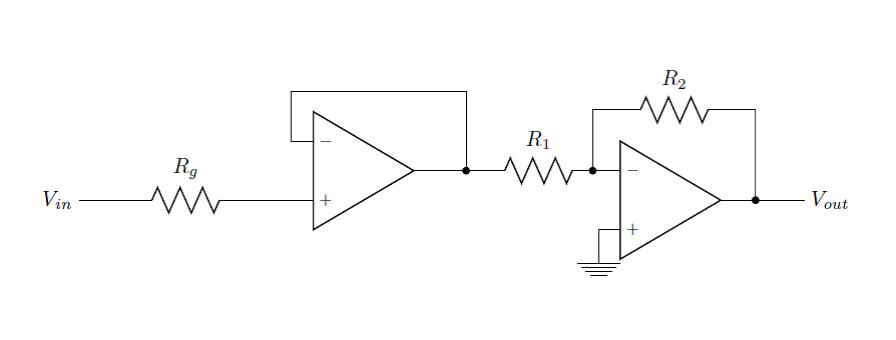
\includegraphics[scale=0.35]{bah}
\end{figure}

Abbiamo fatto prove con diversi valori per $R_g$. Per valori di tale resistenza dell'ordine del centinaio di $k\Omega$ non si è rilevata alcuna differenza dai risultati ottenuti con il circuito invertente collegato direttamente alla scheda di acquisizione (che ha una resistenza interna di 0.1~$\Omega$). Riportiamo i risultati delle prove in una tabella e il fit nel caso $R_g = 2.2 k\Omega$, così da confrontarlo con i risultati ottenuti precedentemente:

\begin{figure}[htp]
\centering
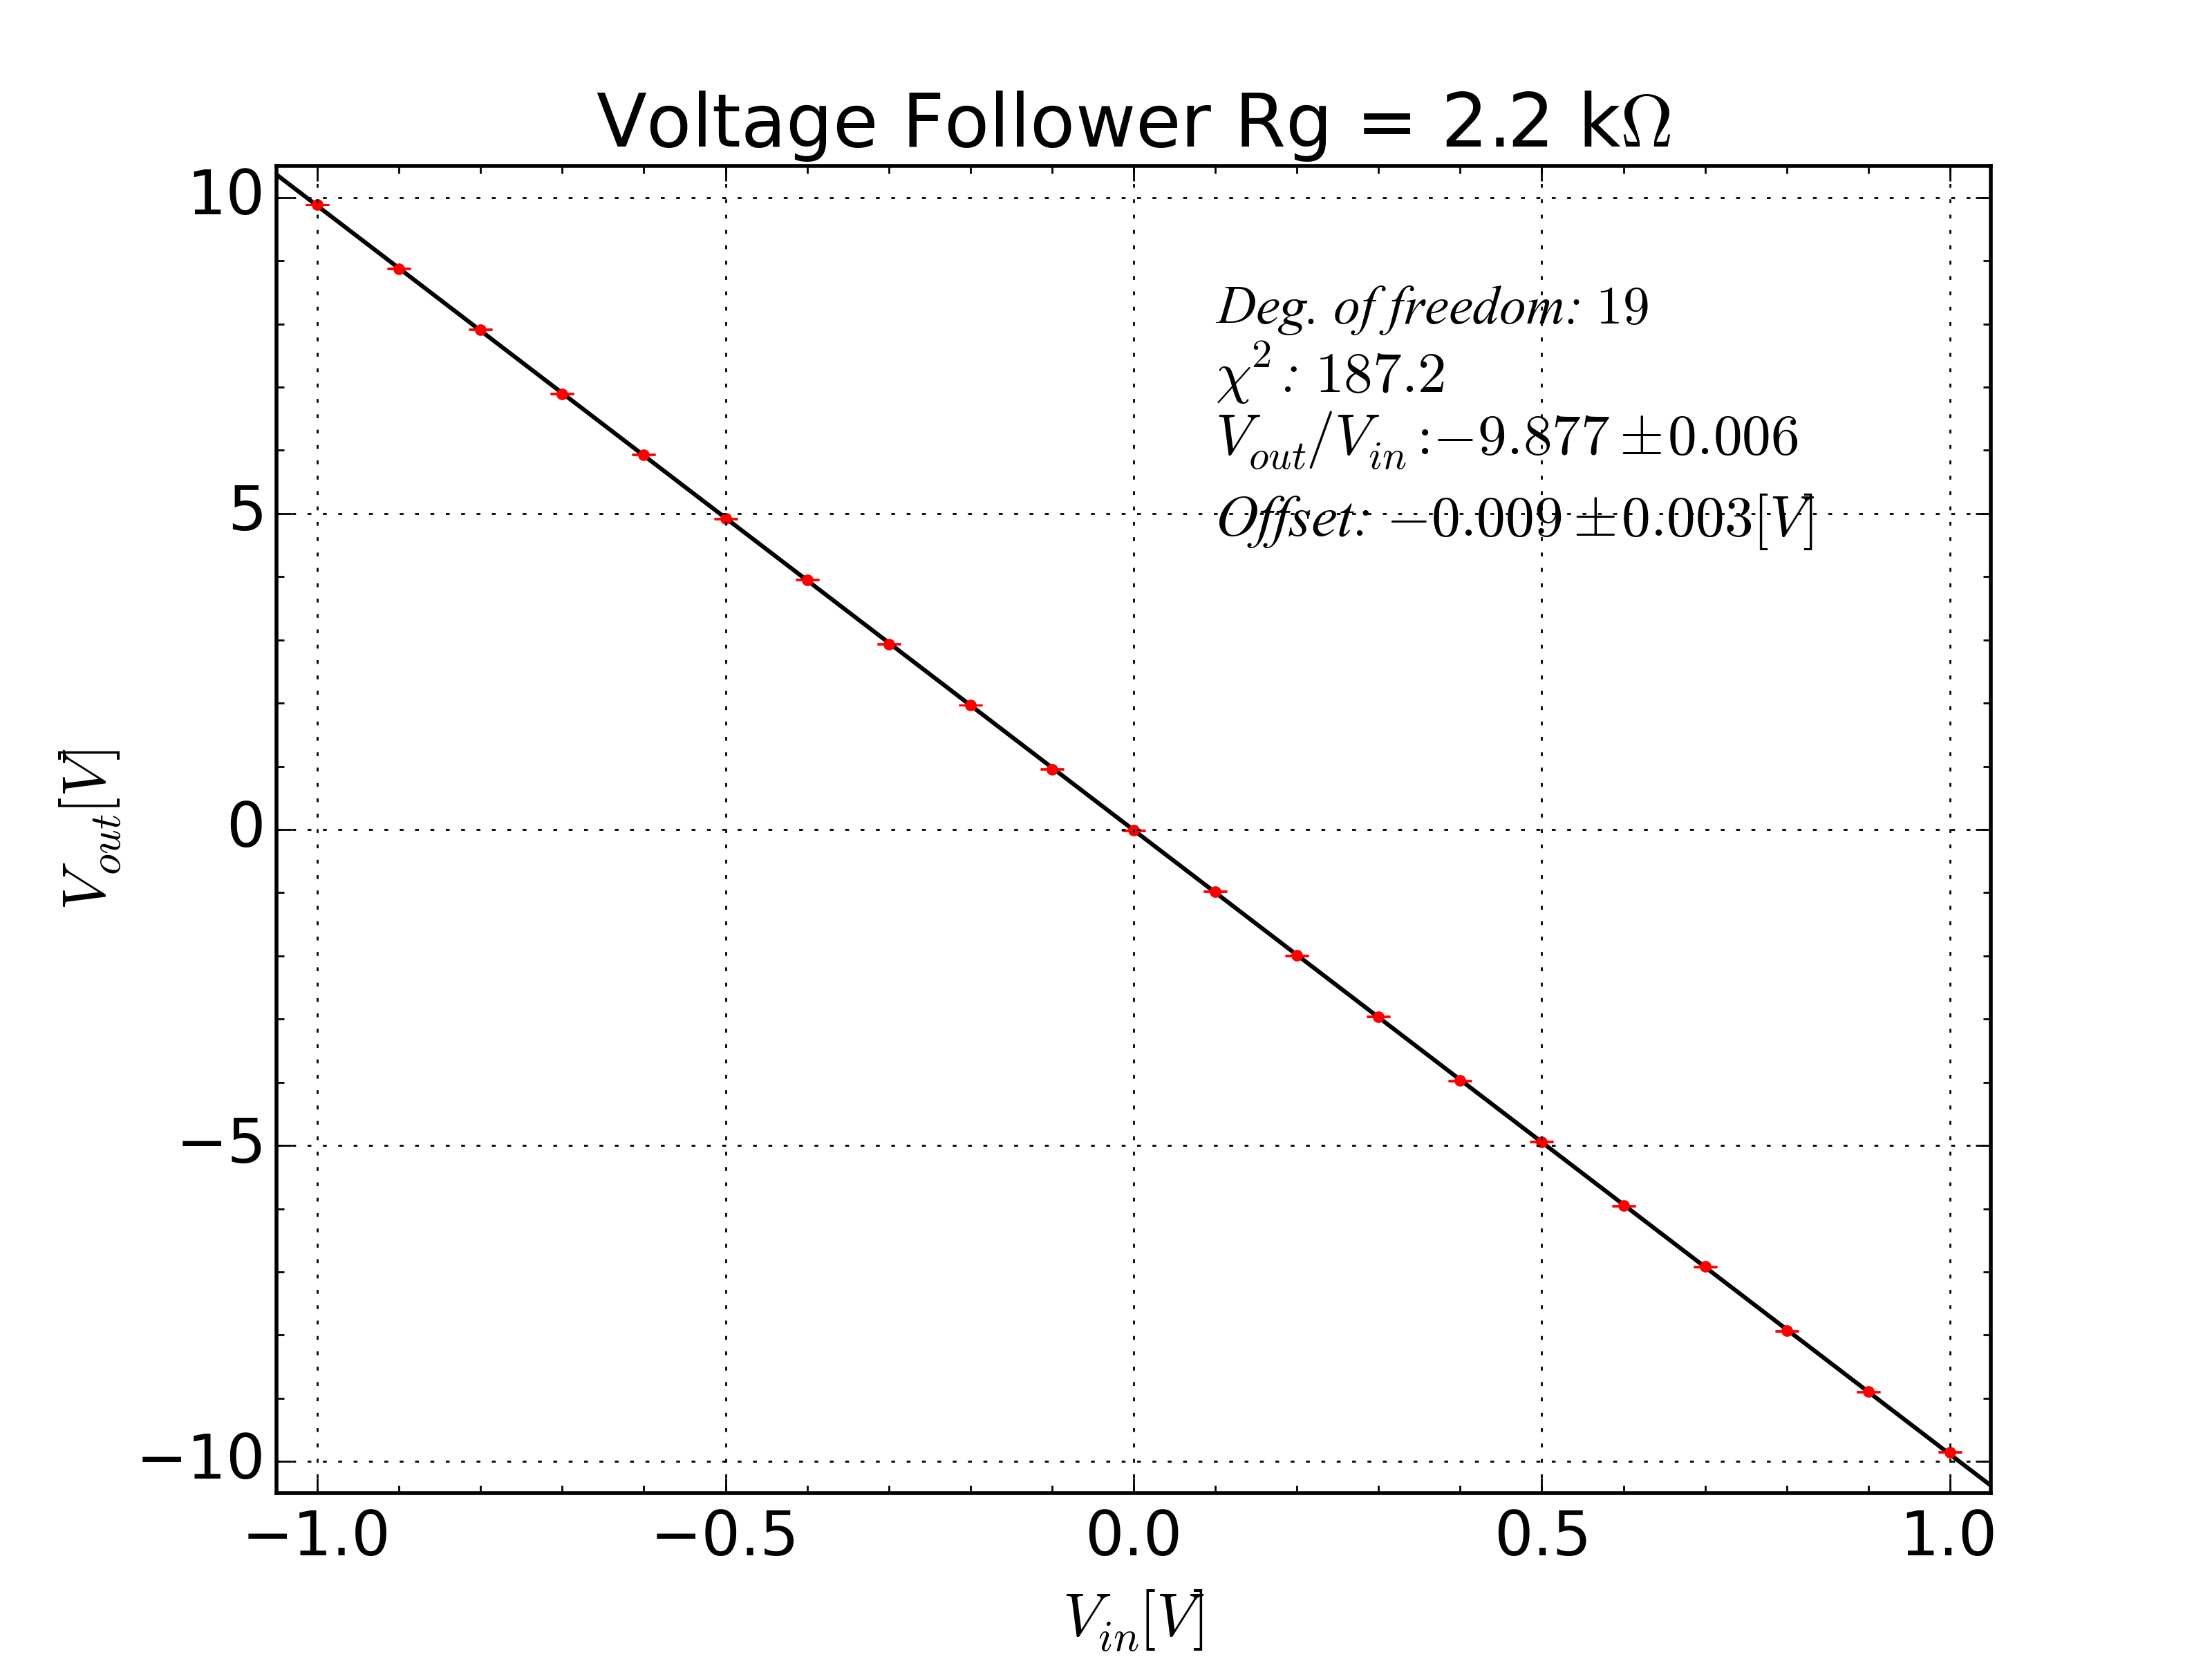
\includegraphics[scale=.35]{fit_follower_1_21_2k_2k_22k}
\caption{Fit follower+invertente con $R_g = 2.2~k\Omega$. I risultati sono in accordo con quelli relativi all'opamp invertente collegato direttamente alla scheda di acquisizione.}
\end{figure}

\begin{center}
\captionof{table}{Dati relativi al Gain e all'offset per resistenze dell'ordine dei 100 ~ $k\Omega$ e inferiore.\\}
\begin{tabular}{|c|c|c|}
\hline 
$R_g (k\Omega)$ & G (-$\frac{R_2}{R_1}$) & Offset (mV) \\ 
\hline 
2.2 & -9.877 $\pm$ 0.006 & -9 $\pm$ 3 \\ 
\hline 
22 & -9.874 $\pm$ 0.005 & -4 $\pm$ 4 \\ 
\hline 
220 & -9.876 $\pm$ 0.005 & 38 $\pm$ 3 \\ 
\hline 
\end{tabular} 
\end{center}

~\\
Si nota che già per $R_g = 220 k\Omega$ si ottiene un offset sensibilmente diverso da zero. Infatti per resistenze maggiori, si nota che all'aumentare della resistenza $R_g$ aumenta l'offset, per di più in modo lineare. Si riporta il fit per $R_g = 2 M\Omega$ e i dati relativi alle altre resistenze impiegate:

\begin{figure}[htp]
%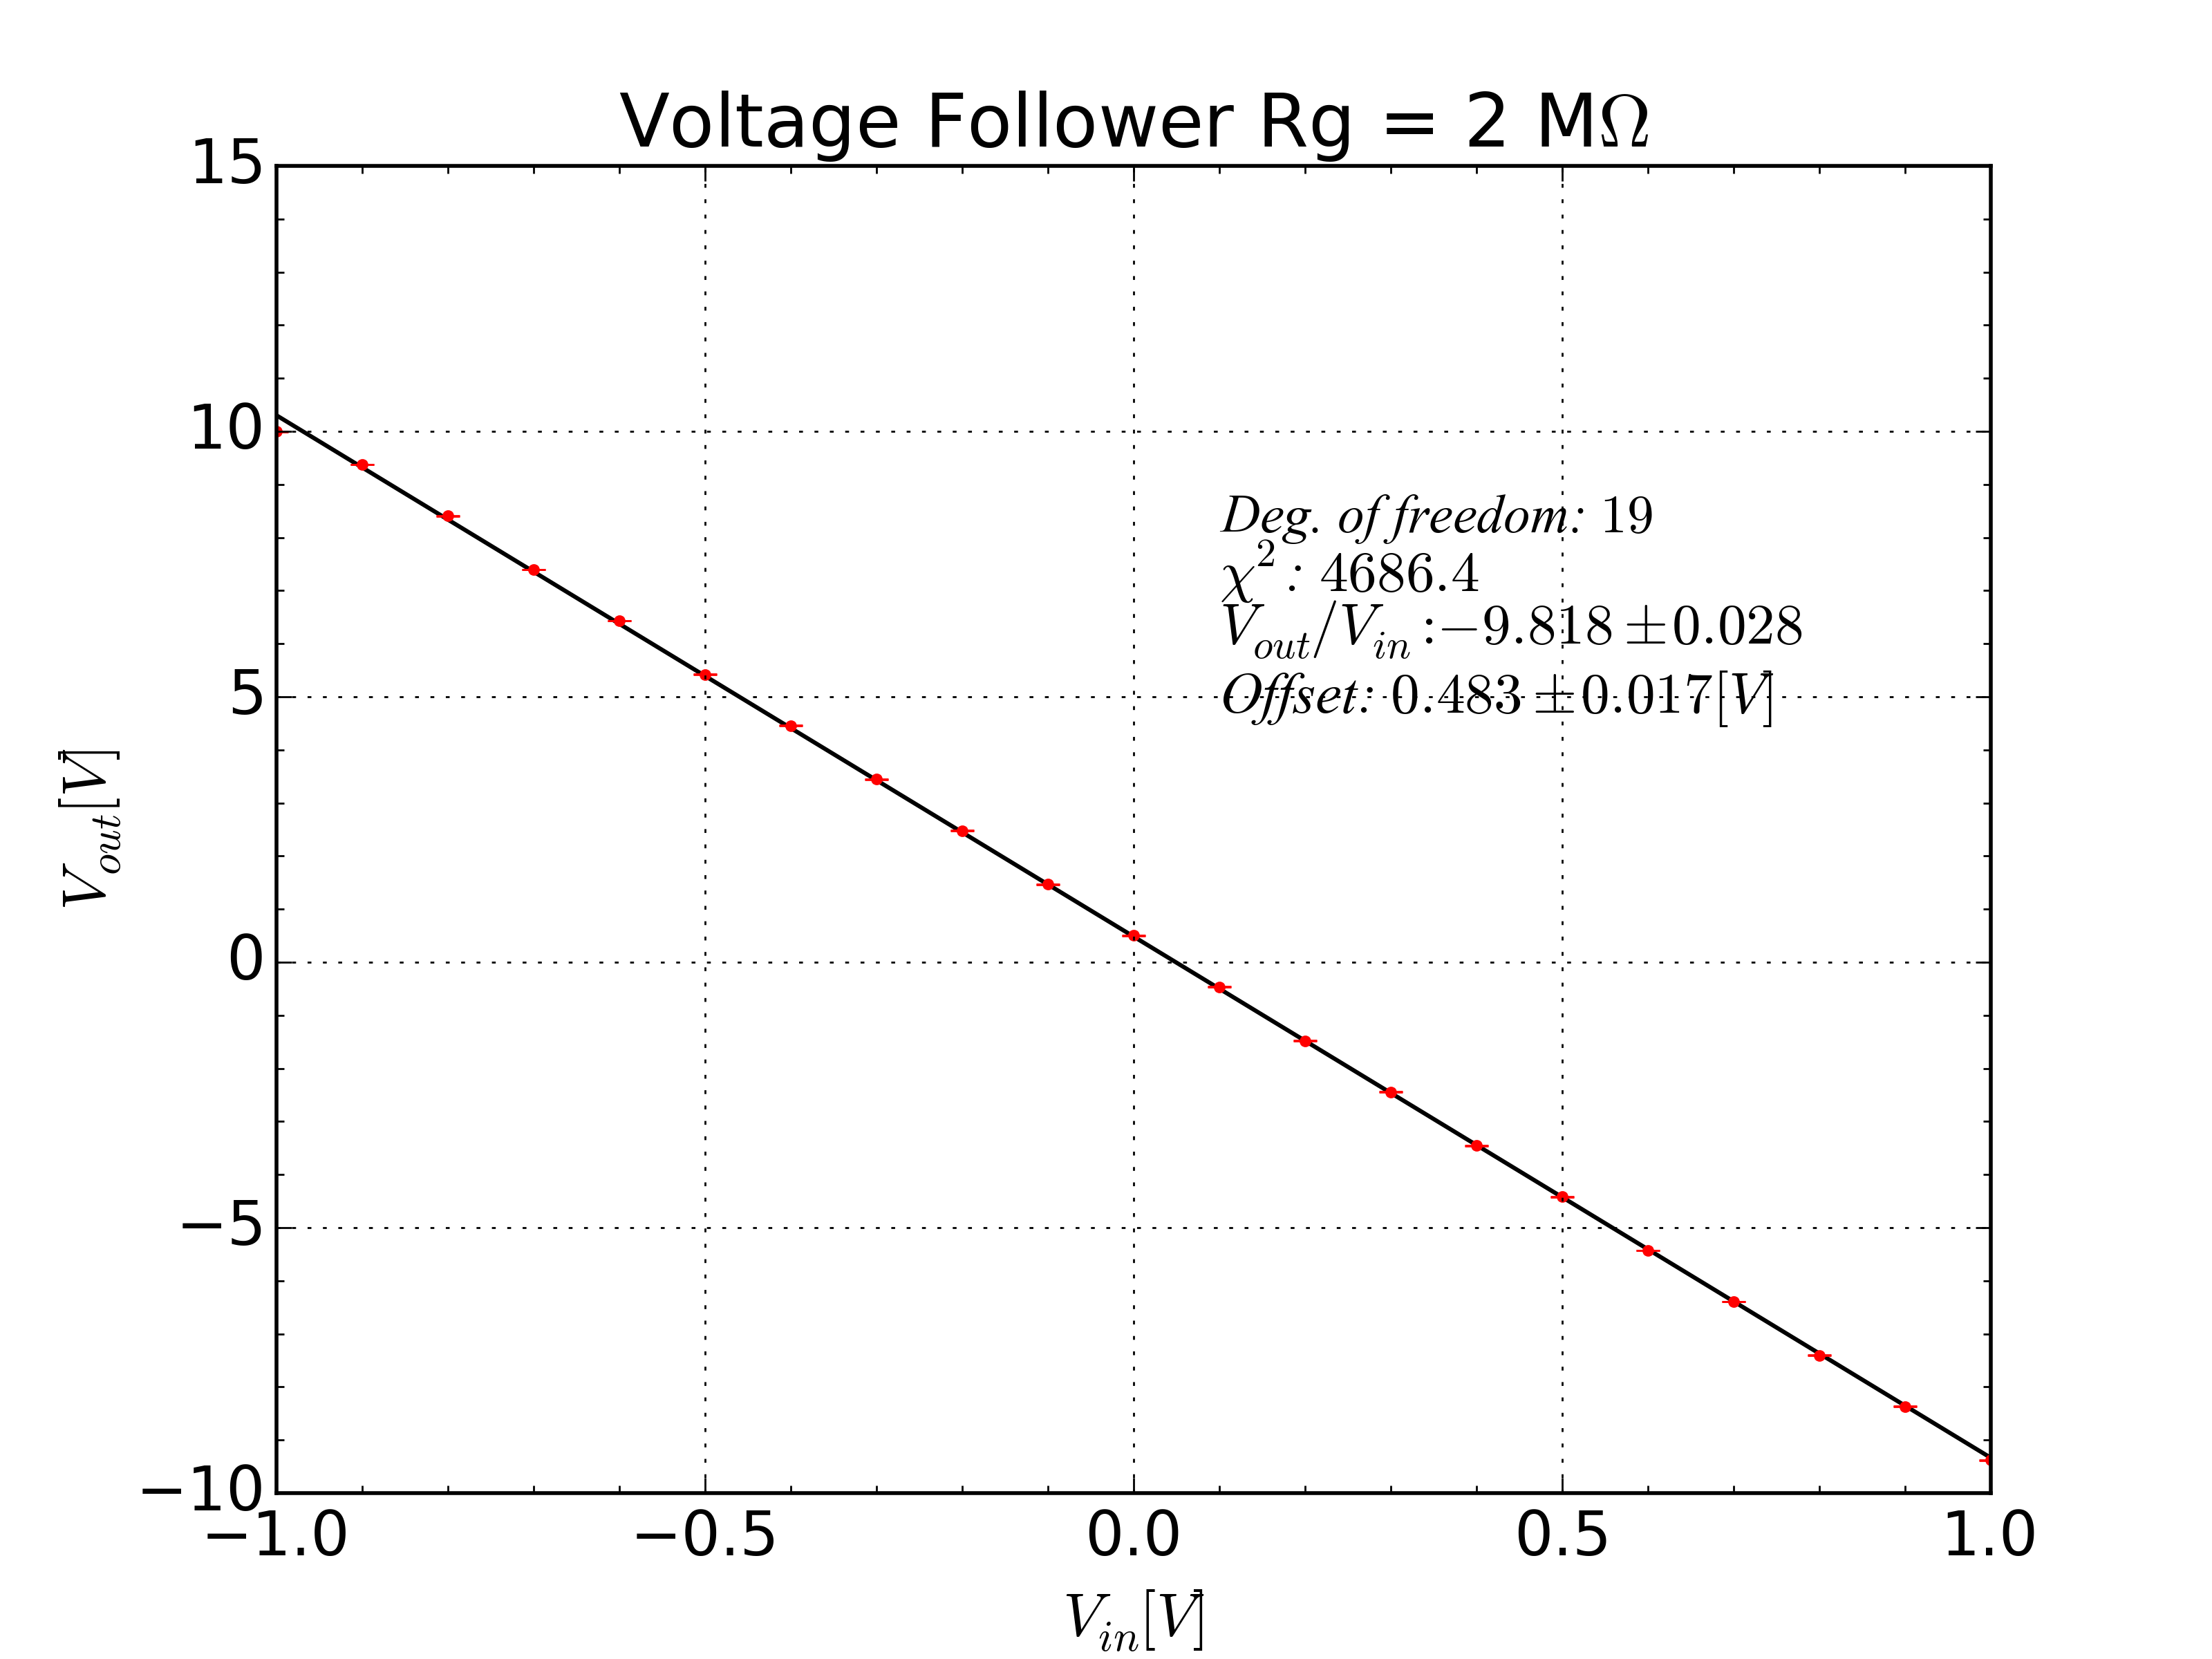
\includegraphics[scale=.4]{fit_follower_1_21_2M_2k_22k.png}
\end{figure}



\begin{center}
\captionof{table}{Dati rrelativi al Gain e all'offset per $R_g$ dell'ordine del $M\Omega$. Si può notare come l'offset aumenti proporzionalmente al valore della resistenza.\\}
\begin{tabular}{|c|c|c|}
\hline 
$R_g (M\Omega)$ & G (-$\frac{R_2}{R_1}$) & Offset (V) \\ 
\hline 
1 & -9.885 $\pm$ 0.007 & 0.205 $\pm$ 0.003 \\ 
\hline 
2 & -9.818 $\pm$ 0.005 & 0.483 $\pm$ 0.017 \\ 
\hline 
3 & -9.869 $\pm$ 0.007 & 0.716 $\pm$ 0.003 \\ 
\hline 
10 & -9.811 $\pm$ 0.010 & 2.208 $\pm$ 0.005 \\ 
\hline 
20 & -9.754 $\pm$ 0.008 & 4.400 $\pm$ 0.004 \\ 
\hline 
\end{tabular} 
\end{center}
~\\
La ragione di tale andamento è da imputarsi al fatto che per questi valori di resistenza, confrontabili con la resistenza in ingresso all'opamp, vengano meno le regole d'oro dell'opamp stesso, tuttavia non si sa in che senso tali regole non siano più valide.\\

Un opamp in configurazione invertente può lavorare come amplificatore di corrente. Dato lo schema in figura infatti:\\

\begin{circuitikz}
\centering
\node[ground] at (5,-0.8) {};
\draw (5,-0.8) to[american current source](5,0.49);
\draw (5,0.49) to[short](6.6,0.49);
\draw (7.79,0) node[op amp]{};
\draw (6.5,0.49) to[short,*-](6.5,1.5);
\draw (6.5,1.5) to[R,l^=$R$](9.2,1.5);
\draw (9,0) to[short](10,0);
\draw (10,0) node[anchor=west]{$V_{out}$};
\draw (9.2,1.5) to[short,-*](9.2,0);
\draw (6.6,-0.49) to[short](6.6,-1);
\node[ground] at (6.6,-1) {};

\end{circuitikz}

~\\
Per la regola della terra virtuale e per il verso fissato in figura per la corrente si ha che:
\begin{equation}
V_{out} = -Ri
\end{equation}

Abbiamo disegnato il circuito in Figura (\ref{fig_tina}) con TINA:

\begin{figure}[htp]
\caption{Circuito disegnato con TINA}
\label{fig_tina}
\centering
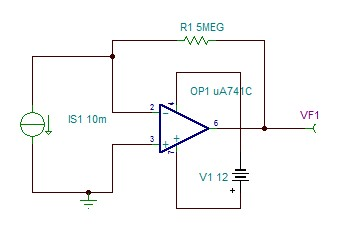
\includegraphics[scale=.4]{CONVERTITORE}
\end{figure}

e abbiamo tracciato la curva caratteristica DC del circuito prima supponendo il generatore di corrente ideale e poi reale con resistenza interna di 1~$M\Omega$. Si è scelto R = 5 $M\Omega$, poiché verrà impiegata in seguito con il diodo.
I grafici ottenuti sono in Figura (\ref{gen_rel}) e (\ref{gen_id}) :\\

\begin{figure}[htp]
\centering
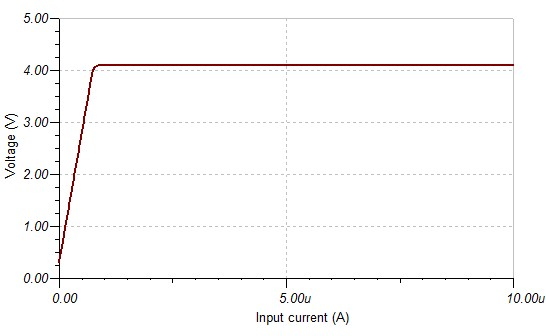
\includegraphics[scale=.35]{convertitore_analysis}
\caption{Generatore reale}
\label{gen_rel}
\end{figure}

\begin{figure}[htp]
\centering
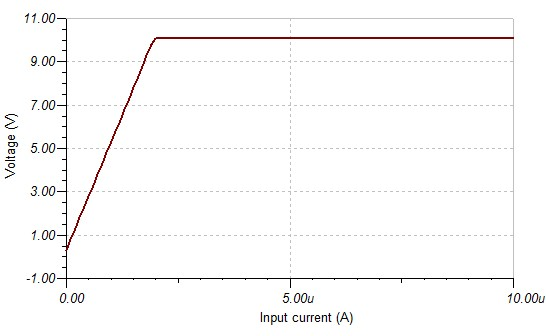
\includegraphics[scale=.35]{convertitore_analysis_infinite}
\caption{Generatore ideale\\}
\label{gen_id}
\end{figure}

In entrambi i casi l'andamento è lineare fino $I\approx 1~\mu A$, con pendenza, stimata prendendo 2 punti e calcolandone il rapporto incrementale, di 5.008 $M\Omega$ nel caso reale, 4.997 $M\Omega$ nel caso ideale, per cui in questo intervallo il circuito risponde come previsto. Per correnti superiori invece già nella simulazione si vede il limite dell'opamp reale. Infatti se si tracciano le d.d.p. ai capi della resistenza e del generatore di corrente, supposto direttamente reale, tramite il circuito di TINA in Figura (\ref{circuito_tina}):


\begin{figure}[htp]
\caption{Circuito per rilevare le tensioni ai capi dei singoli componenti}
\label{circuito_tina}
\centering
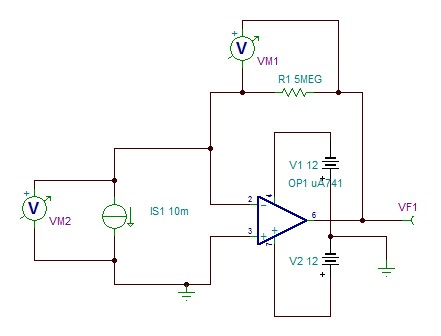
\includegraphics[scale=.4]{newTINA}
\end{figure}

Si ottiene quindi il grafico in Figura \ref{graf_tens}:\\

\begin{figure}[htp]
\centering
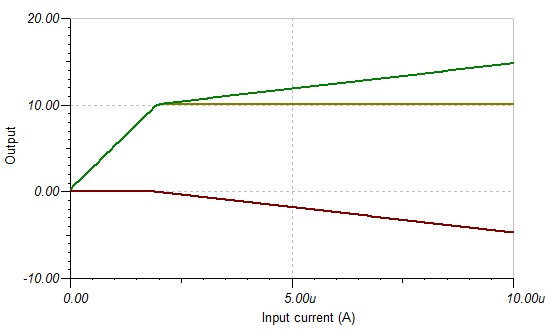
\includegraphics[scale=.5]{immagine3}
\caption{Grafico delle tensioni ai capi del generatore di corrente ($V_A$), della resistenza ($V_R$) e di $V_{out}$\\}
\label{graf_tens}
\end{figure}


Si vede come fino a $I\approx 1~\mu A$, la regola della massa virtuale sia rispettata, in quanto ai capi del generatore di corrente la d.d.p. è nulla, per cui anche agli ingressi dell'op amp, e in tale intervallo $V_R$ aumenta secondo quanto previsto. Per $I\geq 1 \mu A$ invece la seconda regola d'oro dell'op amp non è più valida e inizia a scorrere corrente dentro l'op amp, giustificando il grafico di $V_R$, in modo tale da mantenere un $V_{out}$ costante, anche se non è chiaro il motivo di quest'ultima caratteristica.\\

Si è applicato l'op amp come \textit{transresistance amplifier} per misurare la corrente di saturazione inversa di un diodo. Abbiamo usato il diodo 1N4148 della NXP semiconductors. Dal datasheet disponibile sul sito \url{www.nxp.com} abbiamo ricavato le informazioni per posizionare correttamente il diodo (vedi Figura (\ref{diodo})).

\begin{figure}[htp]
\centering
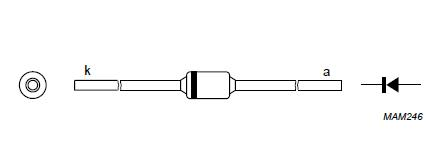
\includegraphics[scale=.45]{dido}
\caption{Schema di polarizzazione del diodo 1N4148 ricavato dal datasheet}
\label{diodo}
\end{figure}


Sul datasheet si legge che:

\begin{itemize}
\item la massima d.d.p. in polarizzazione inversa è 100 V, mentre in diretta è 1 V;
\item dentro il diodo può scorrere al massimo una corrente di 200 mA in continua;
\item la potenza totale dissipata è 500 mW;
\item la temperatura della giunzione non può superare i 200 C, il diodo in sè non deve essere sottoposto a temperature inferiori ai -65 C e superiori ai 200 C;
\item la corrente di saturazione inversa a 20 V è 25 nA;
\item vi sono grafici relativi all'andamento della corrente massima in funzione della temperatura, curva caratteristica a varie temperature, reverse current in funzione della temperatura e capacità del diodo in termini di tensione di polarizzazione inversa.\\
\end{itemize}

Altre informazioni risultano poo chiare come il significato di reverse peak current o voltage e relativi grafici o recovery voltage.\\
Abbiamo realizzato sulla breadboard il circuito di Figura (\ref{op-diod}):\\

\begin{figure}[htp]
\caption{}
\label{op-diod}
\centering
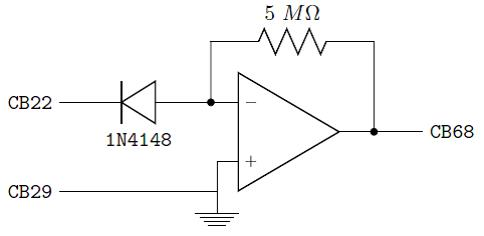
\includegraphics[scale=.4]{diodo}
\end{figure}

Come resistenza abbiamo impiegato un parallelo di due resistenze da 10 $M\omega$. Abbiamo esplorato un intervallo di 10 V a partire da 0 V. I dati restituiti sono raccolti nel grafico (\ref{plotdiodosil}):\\

\begin{figure}[htp]
\caption{}
\label{plotdiodosil}
\centering
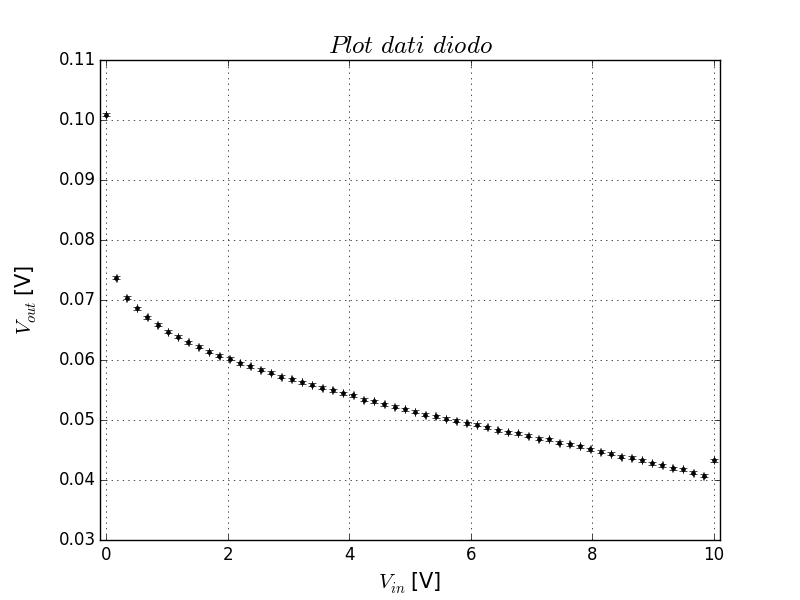
\includegraphics[scale=.35]{plotdiodosil}
\end{figure}

Si nota subito come $V_{out}$ sia costantemente positivo, mentre ci si aspettava una tensione negativa. Ciò lo si può imputare alle condizioni non ideali di lavoro dell'op amp. Infatti per $V_{in} = 0$ V si osserva una tensione $V_{in} = (0.1009 \pm 0.003)$ mV, anziché 0. Abbiamo sostituito il diodo con una resistenza da 10 $M\Omega$ e riavviato l'acquisizione cambiando l'intervallo di tensione in (-1 V, 1 V). I dati ottenuti sono plottati in (\ref{plotdiodores}):\\

\begin{figure}[htp]
\caption{}
\label{plotdiodores}
\centering
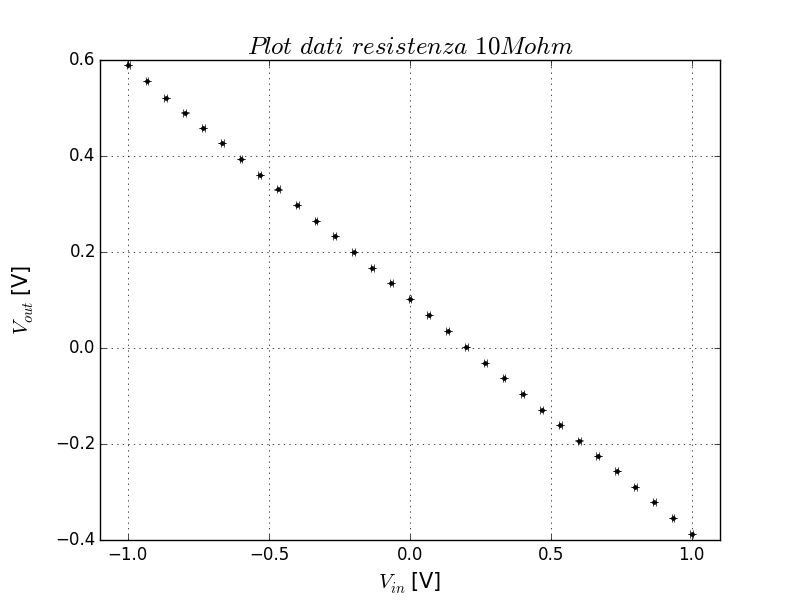
\includegraphics[scale=.35]{plotdiodores}
\end{figure}

Dal confronto fra questo grafico e il grafico precedente si può dedurre che naturalmente l'andamento dei dati sperimentali nel secondo caso è dovuto interamente al diodo, mentre l'offset a $V_{in} = 0$ V interamente all'op amp. Infatti sostituendo il diodo con la resistenza si ottiene che per $V_{in} = 0$ V si ha $V_{out} = (0.1020 \pm 0.0003)$ V, quasi compatibile con il valore ottenuto con il diodo. Per isolare dunque il contributo alla $V_{out}$ dovuto unicamente alla reverse current del diodo si può eliminare tale offset dai dati sperimentali che risultano come nel grafico (\ref{plotdiodo_no_offset}):

\begin{figure}[htp]
\caption{}
\label{plotdiodo_no_offset}
\centering
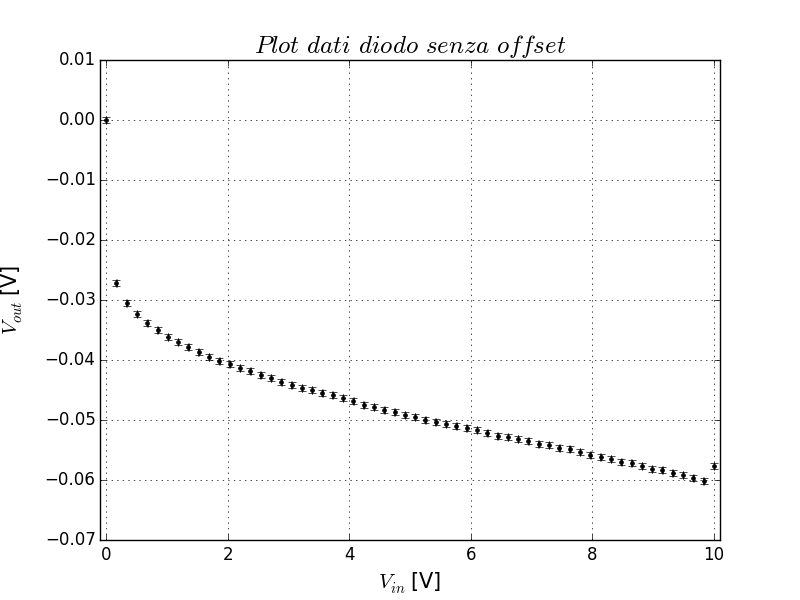
\includegraphics[scale=.35]{plotdiodo_no_offset}
\end{figure}

Un altro aspetto notevole è il fatto che il diodo non arriva mai a saturazione nell'intervallo considerato, in quanto anziché osservare un andamento costante se ne osserva uno lineare, anche se non è chiaro se ciò è dovuto solamente al comportamento reale del diodo o anche all'interazione con l'op amp.\\
Si può dedurre il valore della corrente di saturazione media ad esempio prendendo i dati nella regione ad andamento lineare e facendone media e scarto quadratico medio della media. Il risultato ottenuto è $I_r = (10.2 \pm 1.2)$ nA, in accordo con quanto si legge nel datasheet.\\

Per quanto riguarda il diodo 1N4148, TINA fornisce i 19 parametri di Figura (\ref{dati_Tina}):\\

\begin{figure}[htp]
\caption{}
\label{dati_Tina}
\centering
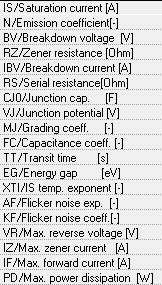
\includegraphics[scale=.7]{dati_Tina}
\end{figure}


Per cui TINA può agire sia sulla corrente di saturazione inversa e permette di regolare effetti ai limiti come la tensione e la corrente di breakdown, la resistenza Zener, oltre che vari valori limite come la massima tensione in polarizzazione inversa, la massima corrente Zener, la corrente in polarizzazione diretta e la massima potenza dissipabile. Il diodo viene anche dotato di una capacità. Rispetto al datasheet, TINA fornisce una reverse current di 1 nA, mentre il datasheet fornisce diversi valori in funzione delle condizioni di lavoro del diodo (nel nostro caso 10 nA). La massima corrente e potenza dissipabile sono notevolmente inferiori rispetto a quelli di TINA.\\

Dopo il diodo al silicio abbiamo impiegato il diodo al germanio OA95, che rispetto al dido al silicio dovrebbe far passare più corrente in polarizzazione inversa. Pertanto per rientrare nel fondo scala della scheda di acquisizione abbiamo sostituito il parallelo di resistenze da 10 M$\Omega$ con resistenze più piccole. Abbiamo impiegato dapprima una resistenza da 220 k$\Omega$, ottenendo i dati plottati in Figura (\ref{plotdiodo_germanio_220k}):\\

\begin{figure}[htp]
\caption{}
\label{plotdiodo_germanio_220k}
\centering
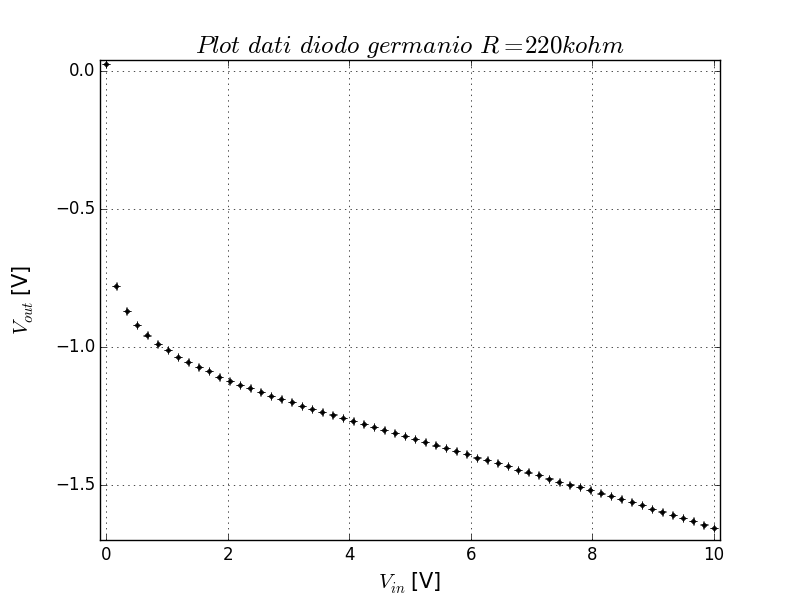
\includegraphics[scale=.35]{plotdiodo_germanio_220k}
\end{figure}

Si nota un andamento identico rispetto al diodo al silicio, per cui entro 10 V neanche il diodo al germanio raggiunge la saturazione. Tuttavia rispetto al diodo 1N4148, l'offset è notevolmente ridotto a (0.0264 $\pm$ 0.0003) V, questo perché si è abbassata sia la resistenza di carico sia quella del diodo che fa passare più corrente. Dunque il comportamento dell'op amp in questo caso è più vicino a quello ideale, il che suggerisce che il fatto che il diodo non raggiunga la saturazione neanche in questo caso si possa imputare principalmente al comportamento reale del diodo. Per la corrente di saturazione media, procedendo come prima si ottiene $I_r = (6.5 \pm 0.7) \mu A$, maggiore di un fattore 600 rispetto al precedente con il diodo al silicio.
\end{document}
